%http://www.latexstudio.net/archives/2234.html
% TikZ 与 pgfplots 结合
% 我们使用 pgfplots 宏包画函数图会方便很多,上面说到的范围过大的问题也不会存在(原生函数作图);pgfplots 提供我们一个 axis 环境,下面给出一个例子:
%-------------------------------------------------------------
% 注意事项:
% pgfplots 没有 sin(\x r) 这种写法,而是使用 deg(x) 将 x 识别为弧度。
% addplot 命令可以为我们创建分段函数,只要确定不同的定义域(参数 domain),设定不同的函数即可。
% 默认地,pgf 并不把坐标系建在原点,为了更符合我们的习惯,需要用到两个选项:
% axis x line=middle
% axis y line=middle
\documentclass[border=4pt]{standalone}

\usepackage{mathpazo}
\usepackage{pgfplots}
\newcommand{\num}{pi}
\pgfplotsset{compat=1.8}
 % define the plot style and the axis style
\tikzset{elegant/.style={smooth,thick,samples=50,magenta}}
 

\begin{tikzpicture}
\draw(0,0)--+(2,-2);
\end{tikzpicture}
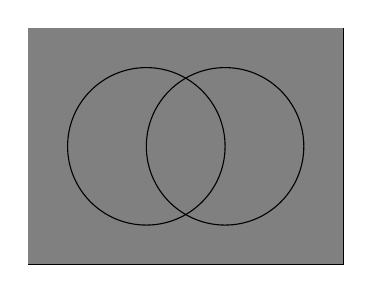
\begin{tikzpicture} \draw (-2, 1.5) rectangle (2, -1.5); \fill[color=gray] (-2,1.5) rectangle (2,-1.5); \draw (-0.5, 0) circle (1); \draw ( 0.5, 0) circle (1); \end{tikzpicture}
\par


\usetikzlibrary{calc,through}
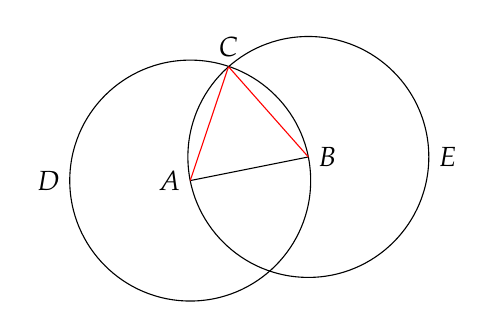
\begin{tikzpicture}[scale=1.2] 
\coordinate [label=left:$A$] (A) at (0,0); \coordinate [label=right:$B$] (B) at (1.25,0.25); \draw (A) -- (B); 
\node (D) [draw,circle through=(B),label=left:$D$] at (A) {}; 
\node (E) [draw,circle through=(A),label=right:$E$] at (B) {}; \coordinate[label=above:$C$] (C) at (intersection 2 of D and E); 
\draw [red] (A) -- (C); 
\draw [red] (B) -- (C); 
\end{tikzpicture}
\par

\begin{tikzpicture} \draw (-2,-0.8) sin (1,1) cos (2,0)\end{tikzpicture}

\begin{tikzpicture}[scale=0.4,line cap=round,line join=round,>=triangle 45,x=1.0cm,y=1.0cm] 
\draw[-latex,color=black,thick] (-7.42,0) -- (13,0) node[above] {$x$}; 
\draw[-latex,color=black,thick] (0,-6.21) -- (0,9)node[right] {$y$}; 
\draw[color=black] (0pt,-10pt) node[right] {\footnotesize $O$}; 
\clip(-7,-6) rectangle (12,5); 
\draw[smooth,samples=100,domain=-pi:pi,thick,variable=\t] plot({2*sec((\t r))},{sqrt(2)*tan((\t r))}); 
\end{tikzpicture}



\end{document}